\documentclass{article}
\usepackage[utf8]{inputenc}
\usepackage[english]{babel}
\usepackage{amsmath}
\usepackage{listings}
\usepackage{graphicx}
\usepackage{comment}
\usepackage{float}
\usepackage{biblatex}
\usepackage{lscape}
\usepackage{csquotes}
\usepackage{multirow}
\addbibresource{bibliography.bib}
\usepackage[a4paper,pdftex,bottom=20mm, width=160mm]{geometry}
\setlength{\parindent}{0pt}
\setlength{\parskip}{1em}

\title{
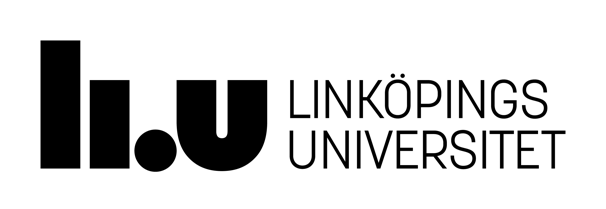
\includegraphics[scale=1.5]{liu_logga.png} \\
\vspace{2.0cm} \textbf{Software Quality Assurance Plan} \\
 \endgraf\rule{\textwidth}{.4pt}
  \large \textbf{TDDC88 - Project - Company 3}\\
   }

\author{
% Add your full name here
    Emma Strömberg -- Strategic Product Owner \and 
    Adrian Redfors -- Technical Writer \and 
    Anton -- Testing Lead \and 
    William -- Analysis Lead \and 
    Andreas -- Deployment Lead \and 
    Olle -- Process Manager \and 
    Chang -- Architecture
}
\date{\today}

\section{Information for Authors}
Dear contributors to the Quality Assurance Plan,

Thank you for your participation in creating this crucial document for our TDDC88 project. As we aim for grade 5, your input is vital to ensure a comprehensive and high-quality plan. Please note the following guidelines:
\begin{itemize}
    \item Deadline: The initial draft of your assigned section is due by [2024-10-4 \textit{may change}]. This allows time for review and integration before our next milestone. Note that not all parts f your section can be completed by this time. 
    
    \item Section Ownership: Your name has been assigned to a specific section. You are responsible for the content and timely completion of that section.
    
    \item Content Expectations: Aim for clarity and thoroughness. Each section should be approximately 300-500 words, but prioritize quality over quantity. Include specific, actionable details relevant to our project.
    
    \item Grade 5 Focus: We are aiming for grade 5. Ensure your section demonstrates:
    \begin{itemize}
        \item Integration with overall development processes
        \item Support for continuous improvement
        \item Forward-thinking approaches to quality assurance
    \end{itemize}
    
    \item Collaboration: While you're responsible for your section, feel free to consult with team members. 
    
    \item Version Control: Adrian will manage version control. Submit your updates in Overleaf by Wednesday evenings to be included in the weekly GitLab update.
    
    \item Questions: If you have any questions or need clarification, please contact Emma (Strategic Product Owner) or Adrian (Technical Writer).
\end{itemize}
Remember, this document is crucial for our project's success and our course grade. Your expertise and diligence are greatly appreciated.
Thank you for your commitment!
\textit{*Emma - Strategic Product Owner \& Adrian - Technical Writer}

\vspace{1cm}
\textbf{Sections and Responsible Authors:}
\begin{itemize}
    \item Document Structure and Ownership: \textit{Adrian TechnicalWriter}
    \item Testing Strategy: \textit{Anton TestingLead}
    \item Traceability: \textit{William AnalysisLead}
    \item Continuous Integration and Delivery: \textit{? Andreas DeploymentLead ?}
    \item Bug Tracking and Resolution: \textit{? Anton TestingLead ?}
    \item Internal Quality Practices: \textit{Olle ProcessManager}
    \item Change Management: \textit{*Olle* ProcessManager}
    \item Process Evaluation and Improvement: \textit{Emma StrategicManager}
    \item Future Development and Operations: \textit{Chang Architecture}
    \item Implementation and Verification: \textit{Emma StrategicManager}
\end{itemize}

\begin{document}

\maketitle

\newpage
\tableofcontents
\newpage

\section{Introduction}
This Software Quality Assurance (SQA) Plan is a crucial document for our TDDC88 project, aiming to ensure the highest quality standards in our software development process. As we are targeting grade 5, this plan incorporates all necessary components to meet and exceed the course requirements.

The purpose of this document is twofold:
\begin{enumerate}
    \item To provide a comprehensive framework for maintaining and improving software quality throughout our development lifecycle.
    \item To clearly communicate responsibilities and expectations to all team members, ensuring a coordinated effort towards achieving our quality goals.
\end{enumerate}

This plan is designed to be a living document, regularly updated to reflect our evolving practices and lessons learned. Each section outlines specific quality assurance activities, their purpose, and the individuals responsible for their implementation.


\section{Document Structure and Ownership}
\textit{Responsible: *Adrian* TechnicalWriter}

This section details the overall structure of the SQA plan, ensuring it is well-organized, easily navigable, and accessible to all team members. The structure is designed to support continuous improvement and integration with our overall development processes.

\subsection{Document Structure}
The SQA plan is organized into clearly defined sections, each corresponding to a key aspect of our quality assurance process. This structure ensures:

\begin{itemize}
    \item Easy navigation and quick reference for team members
    \item Clear delineation of responsibilities
    \item Logical flow from high-level strategy to specific implementation details
    \item Facilitation of regular updates and continuous improvement
\end{itemize}

\subsection{Authorship}
Each section owner is responsible for authorship of their own section. This decentralized approach ensures that the content is created and maintained by those with the most relevant expertise. Responsibility for formatting and information sharing about the Quality Assurance plan is shared between Emma and Adrian:

\begin{itemize}
    \item \textit{Emma - Strategic Product Owner}: Responsible for stakeholder communication and ensuring alignment with project goals
    \item \textit{Adrian Technical Writer}: Responsible for version control, document formatting, and maintaining overall document consistency
\end{itemize}

This collaborative approach supports continuous improvement by leveraging diverse expertise and maintaining clear lines of communication.

\subsection{Version Control System}
To support requirements for integration with development processes and continuous improvement, we implement a robust version control system:

\begin{itemize}
    \item The document is primarily edited in Overleaf, a collaborative LaTeX editor, shared with all responsible authors
    \item Weekly updates are made to GitLab every Thursday at 8am, before the weekly company meeting
    \item Each GitLab update includes:
    \begin{itemize}
        \item The latest version of the document
        \item A brief note detailing changes made since the last update
        \item Any relevant discussion points or decisions made regarding the document
    \end{itemize}
    \item Special updates are made before tollgate meetings, taking precedence over the regular weekly schedule
    \item GitLab's version history feature is used to track changes over time, supporting our continuous improvement efforts
\end{itemize}

\subsection{Continuous Improvement and Integration}
This structure supports continuous improvement and integration with overall development processes by:

\begin{itemize}
    \item Enabling real-time collaboration through Overleaf
    \item Providing a clear schedule for updates, aligning with project milestones and meetings
    \item Utilizing GitLab's features to track changes and facilitate discussions
    \item Ensuring the SQA plan evolves alongside the project, reflecting current best practices and lessons learned
    \item Facilitating easy access and reference for all team members, promoting a culture of quality throughout the development process
\end{itemize}

It is our belief that by maintaining this structured approach to document management and version control, we ensure that our SQA plan remains a living, evolving guide that directly supports our commitment to high-quality software development and continuous process improvement.

\section{Testing Strategy}
\textit{Responsible: *Anton* TestingLead}

Outline a comprehensive testing strategy that covers:

\begin{itemize}
    \item Detailed test plan covering unit, integration, system, and acceptance testing
    \item Description of testing tools to be used
    \item Process for reporting and analyzing test results
    \item Strategy for continuous testing throughout the development lifecycle
\end{itemize}

For grade 5, include how the testing strategy supports continuous delivery and how it integrates with other quality assurance processes.

\section{Traceability}
\textit{Responsible: *William* AnalysisLead}

Describe the approach for maintaining traceability between requirements, system design, and test documents. Include:

\begin{itemize}
    \item Tools and techniques used for traceability
    \item Process for updating and maintaining traceability links
    \item How traceability supports quality assurance activities
\end{itemize}

For grade 5, explain how traceability contributes to continuous improvement and supports future development considerations.

\section{Continuous Integration and Delivery}
\textit{Responsible: *Andreas* DeploymentLead}

Detail the implementation of continuous integration (CI) and continuous delivery (CD) practices:

\begin{itemize}
    \item CI/CD pipeline description
    \item Tools used for automation
    \item Integration with testing and other quality assurance processes
    \item Frequency of builds and deployments
\end{itemize}

For grade 5, emphasize how CI/CD contributes to overall software quality and supports rapid, reliable software delivery.

\section{Bug Tracking and Resolution}
\textit{Responsible: *Anton* TestingLead}

Outline the bug tracking system and processes:

\begin{itemize}
    \item Selected bug tracking tool
    \item Process for reporting, prioritizing, and assigning bugs
    \item Workflow for bug resolution and verification
    \item Metrics for tracking bug trends and resolution efficiency
\end{itemize}

For grade 5, describe how bug tracking data is used to drive continuous improvement in development practices.

\section{Internal Quality Practices}
\textit{Responsible: *Olle* ProcessManager}

Detail internal quality assurance practices:

\begin{itemize}
    \item Procedures for internal inspections of all documents
    \item Process for internal walk-throughs, including pre-tollgate meeting reviews
    \item Schedule and format for regular quality assurance meetings
\end{itemize}

For grade 5, explain how these practices contribute to a culture of quality and continuous improvement within the team.

\section{Change Management}
\textit{Responsible: *Olle* ProcessManager}

Describe the processes for handling and documenting changes:

\begin{itemize}
    \item Change request procedure
    \item Impact assessment process
    \item Approval and implementation workflow
    \item Documentation and communication of changes
\end{itemize}

For grade 5, emphasize how change management supports agility while maintaining quality standards.

\section{Process Evaluation and Improvement}
\textit{Responsible: *Emma* StrategicManager}

Outline the approach for continuous evaluation and improvement of QA processes:

\begin{itemize}
    \item Schedule and method for regular evaluation of QA processes
    \item Metrics for measuring process effectiveness
    \item Procedure for implementing and documenting improvements
    \item Feedback loops from team members and stakeholders
\end{itemize}

This section is crucial for achieving grade 5, demonstrating a commitment to ongoing enhancement of quality practices.

\section{Future Development and Operations}
\textit{Responsible: *Chang* Architecture}

Address considerations for future scalability and long-term maintenance:

\begin{itemize}
    \item Architectural considerations for future scalability
    \item Plans for long-term maintenance and support
    \item Strategies for adapting QA processes as the project evolves
\end{itemize}

This forward-looking section is essential for grade 5, showing consideration of the project's long-term quality needs.

\section{Implementation and Verification}
\textit{Responsible: *Emma* StrategicManager}

Describe how the SQA plan will be implemented and verified:

\begin{itemize}
    \item Steps for rolling out the plan to the team
    \item Training or orientation sessions for team members
    \item Regular cross-checks against course grading criteria
    \item Periodic reviews with supervisors to confirm alignment
    \item Internal audits of QA practices against the plan
\end{itemize}

This section ensures that the plan is not just a document, but an active part of the development process, which is crucial for grade 5.

\section{Conclusion}
This SQA Plan provides a comprehensive framework for ensuring high-quality software development in our TDDC88 project. By following this plan and continuously improving our processes, we aim to deliver a superior product while meeting all requirements for grade 5 in the course.

All team members are expected to familiarize themselves with this plan and actively contribute to its implementation. Regular reviews and updates will ensure that our quality assurance practices remain effective and aligned with project goals throughout the development lifecycle.

\end{document}